\documentclass[12pt]{article}
\usepackage{fancyref}
\usepackage{hyperref}
\usepackage{bibspacing}
\usepackage{graphicx}
\usepackage{caption}
\usepackage{subcaption}
\title{Iris Recognition}
\author{
    Richard Hwang
    \and
    Sharad Vikram
    \and
    Andy Zeng
}
\date{\today}

\begin{document}
\maketitle

\begin{abstract}
Iris recognition is a form of biometric identification performed with computer vision. The iris is an internal organ whose texture is randomly determined during embryonic gestation. It is flat and its texture is relatively stable, as the iris is protected from external harm.  All these features make it a very viable form of biometric recognition. We use an ellipse-fitting technique for iris segmentation, rectify the irises to rectangular coordinates, and feed the irises into a feature extractor. We use various features, such as HOG, DAISY, and a random forest classifier to obtain a 0\% error on the MIU dataset.

\end{abstract}

\newpage

\section{Introduction}
\label{sec:intro}
The iris is a structure in the eye that responsible for controlling the size of the pupil. The iris is responsible for "eye color". It is unique to a given person and also does not change. \cite{wildes} Therefore, it is possible to identify individuals completely based on images of their irises.

Iris recognition can be divided into several sections. Given an image of an eye, we first perform iris localization, which can be found in ~\fref{sec:local}. This gives us the coordinates and dimensions of the iris in the image. The next step is iris segmentation, which can be found in \fref{sec:segment}. This extracts the iris from the image and converts it into a rectangle. This rectangular image is used in the final section, iris recognition, which is found in \fref{sec:recog}.

\section{Related Work}
\label{sec:related}
Iris segmentation in state of the art techniques currently uses Fourier methods to account for eyelid occlusions. They also use statistical methods to account for eyelashes. \cite{daugman2}
Features involve using Hamming distance between 2-D Gabor wavelet features to uniquely identify irises. \cite{daugman} \cite{daugman2} Other methods involve using circular symmetric filters to extract features. \cite{ma}

\section{Dataset}
We chose to work with the Multimedia University (MMU) iris database, contributing a total of 450 images, 5 images per iris, 2 irises per subject. All images were taken using the LG IrisAccess 2200 at a range of 7-25 centimeters. We chose this particular dataset over the others we found online for the following reasons:
\begin{itemize}
\item[1.] It was free.
\item[2.] Due to some privacy issues, most iris datasets require lengthy registration processes, official paperwork, and administrative contacts. However, we had no trouble acquiring this dataset within a few days.
\item[3.] Most datasets offer 3 or fewer images per iris. This particular dataset provides 5 images per iris, giving our machine learning algorithms some functional ease.
\end{itemize}

The largest drawback encountered from using this dataset was the low resolution across all iris images. Post iris localization algorithms performed over the MMU dataset return iris radii of approximately 30 pixels, where as state-of-the-art equipment allows the collection of pixel radii from 80 up to 130+ pixels. This undoubtedly had some effect on the results obtained from the particular feature extraction methods used for this project. 

\section{Localization}
\label{sec:local}
We broke localization into two stages: pupil localization and iris localization.

The visual consistency of pupil color and contour allows for reliable methods of computing the center of the iris. Many iris recognition papers explore a variety of pupil localization algorithms; some methods trade off accuracy for speed, and vice versa. Since running time was not a concern for our application, we went about approaching this problem with circular hough transforms as opposed to convolution. Taking advantage of the pupil's low saturation, we can reasonably filter out everything but the darkest portions of the original grayscale image (pupil, eyelashes, eyebrows, moles), generating a binary image based a low pixel intensity thresholding value. The size of the blob representing the pupil post binary conversion is typically much larger than the size of detected noise (eyelashes, eyebrows, moles, etc), which can then be filtered out from the binary image by removing all blobs possessing a pixel area below some reasonable value. Then using circular Hough transform across the binary image with a reasonable pupil radius range estimate, we can obtain the circle that returns the largest magnitude of accumulator array peaks over the isolated binary pupil blob - giving us a very good estimate of the pupil radius and location.


Following a slight gaussian blur, we applied canny edge detection over the original grayscale image to pick up the edges between the iris and the sclera. We then projected rays in an outward fashion from the center of the pupil in the directions 0 degrees to -45 degrees and -135 degrees to -180 degrees (because the edges of the iris are more likely to be located in those regions). The point at which the very first edge that each ray hits beyond the pupil radius was then saved as a point of interest. The points of interests were collected and the best fit ellipse was computed mathematically. The parameters of any simple ellipse (without taking into account orientation) follows from the equation: $\frac{(x-x_1)^2}{a^2} + \frac{(y-y_1)^2}{b^2} = 1$. Since the center of the ellipse is a static value, we defined our optimization formula as a function that takes in two parameters, $a$ and $b$ values (width and height respectively), and returns the sum squared distances between the points of interest and the points of the projected ellipse computed from the a and b values. This essentially gives us a function that returns a lower positive value depending on how closely a particular ellipse fits the set of points of interest. We can compute the a and b values that return a local minimum for this particular function, giving us the best fit ellipse across the set of points. Because the ratio of the radius of the pupil to the radius of the iris is typically 0.4 to 0.8, we penalize points of interests within this optimization function based on how far they are from this range. Across the entirety of the MMU dataset we worked with, this method of iris localization worked very well.


\section{Segmentation}
\label{sec:segment}
Taking the computed ellipse of the iris, we transformed the image such that the ellipse becomes a circle (as a quick hack to remove subtle camera distortions), and we transformed the image from a polar coordinate system to a cartesian coordinate system, localizing the iris from the rest of the image. Sorting the pixel intensities within the iris images and removing the extreme pixel intensities also allows for the filtering of additional noise caused by skin and eyelashes. This gives us a clean rectangular image of the iris to work with for the purpose of feature extraction and comparison. 

\section{Preliminary results}
\label{sec:preliminary}

Using a basic set of features, we used a 1-nn classifier to run some preliminary tests on the dataset. The results are shown below.\\

\begin{tabular}{| c | c |}
\hline
Features & Error Rate\\
\hline
Raw pixels & 0.767 \\
\hline
5x5 Blocks of Average Pixel Intensities & 0.869 \\
\hline
HOG & 0.119 \\ 
\hline
\end{tabular}\\

No rejection policy was explored for these preliminary testing algorithms.
\section{Hamming distance}
\label{sec:hamming}

Another approach we used was inspired by John Daugman's influential iris detection paper, "How Iris Detection works". \cite{daugman}  We created an {\tt IrisCode} for an iris by calculating the gradient for the iris, and, for each pixel, mapping the direction into two bits representing which quadrant it is in.  We generated an {\tt IrisCode} for each subject using their first image, and this was the subject’s unique identifier.

To classify whether a given iris matched a known iris, we calculated the Hamming distance, the number of different bits, between their IrisCodes.  If the distance was below a threshhold, we said the irises match.  To determine an appropriate theshhold, we trained with two iris images per subject. We created a utility function $f(i,j) = \{tp:1, fp:1, fp: -5, fn:-1\}$.  We then found a threshhold that minimized this utility function applied to all pairs of irises.

Once we found a threshold, we tested on the remaining two iris images per subject. Using this method, we attained $precision=1.0$ and $recall=0.848$ for an $F_1=0.918$.  

Importantly, we had no false positives, which would constitute a security breach.  However, recall can definitely be improved.  Upon inspecting the false negatives, we see most of them had skin and eyelash artifacts from segmentation.  We believe that if we remove these sources of noise we should see a large improvement in performance.

\section{Machine Learning-based Recognition}
\label{sec:recog}
We were able to successfully localize and segment all the images of irises in the MMU dataset. These rectified images were then used as the source of features for a machine learning classifier.

We experimented with several sets of features:
\begin{itemize}
\item[1.] Raw pixels (brightness values)

We took the pixels of the image and concatenated them into one long feature vector of length 7752.
\item[2.] Textons \cite{malik}

We used 25 5x5 texton cluster centers as a basis of generating histograms as features.

\item[3.] PHOG

We computed several histograms of oriented gradients (window sizes 1,2,3,4) and concatenated those into a feature vector

\item[4.] DAISY \cite{daisy}

We computed DAISY features over the image and used them as the feature vector.

\end{itemize}

We split the dataset into 300 training, 150 testing. Here are the results.

\begin{tabular}{| c | c | c |}
\hline
Classifier & Features & Error \\ \hline
SVM & Raw pixels & 0.08 \\ \hline
SVM & Raw pixels + textons & 0.08 \\ \hline
SVM & PHOG & 0.0267 \\ \hline
Random Forest (500 trees, entropy) & DAISY & 0.00 \\ \hline
\end{tabular}

\begin{figure}
  \begin{tabular} {  c  c  c  }
    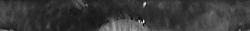
\includegraphics[width=0.3\textwidth]{img/fail-0.png} &
    
\includegraphics[width=0.3\textwidth]{img/fail-1.png} &
    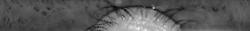
\includegraphics[width=0.3\textwidth]{img/fail-2.png} \\
    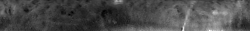
\includegraphics[width=0.3\textwidth]{img/fail-3.png} &
    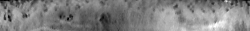
\includegraphics[width=0.3\textwidth]{img/fail-4.png} &
    
\includegraphics[width=0.3\textwidth]{img/fail-5.png} \\
    
\includegraphics[width=0.3\textwidth]{img/fail-6.png} &
    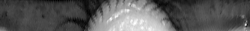
\includegraphics[width=0.3\textwidth]{img/fail-7.png} &
    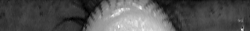
\includegraphics[width=0.3\textwidth]{img/fail-8.png} \\
    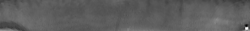
\includegraphics[width=0.3\textwidth]{img/fail-9.png} &
    &
    \\
  \end{tabular}

  \caption{Error cases for raw pixel SVM}
  \label{fig:fail}
\end{figure}


The failure cases for the SVM are presented in \fref{fig:fail}.

\section{Conclusion}
\label{sec:conclusion}

Our machine learning methods were able to bring down our error on the dataset to 0\%. These results are comparable to current SOTA techniques on the dataset and are very encouraging. The variety of features we experimented with show that general computer vision techniques are effective in iris recognition, whereas most related work uses new, domain-specific techniques. 

\section{Future Work}
\label{sec:future}

The dataset we were working with was convenient in that it had images with good lighting, with not too much noise. However, it was also a small dataset. To further benchmark our methods, we could test them on larger, more noisy datasets and see if the computer vision techniques we used will work on tougher data. Other areas to look into would be using more advanced features, such as the Fourier features discussed before and comparing their results to other techniques, and also look into incorporating Hamming distance techinques with the machine learning we performed.

\bibliographystyle{abbrv}
\bibliography{paper}

\end{document}
